\subsection{Benutzersimulation}

Um die Funktionalität der Anwendung eindeutig festzustellen werden typische Benutzeraktionen simuliert und die Ergebnisse an Nagios übermittelt.

Typische Aktionen sind das Einchecken eines Bildes, Suche nach einem Bild und schließlich die Anforderung des Originalbildes und der konvertierten Bilder.
%Benutzertätigkeiten, Handlungen

Da Nagios standardmäßig ein Plugin periodisch jede fünf Minuten aufruft, würde sich die Festplatte und die Datenbank des \gls{OracleUCM}-Servers im Laufe der Zeit an ihre Kapazitäten stoßen.
Daher werden nach der Anforderung und Überprüfung der Bilder alle Testbilder vom Server entfernt.
Ein Testbild soll per Web Service an den Server geschickt und eingecheckt werden.
Mit der Suche nach dem Testbild und der Anforderung der konvertierten Bilder kann die Funktionalität der Anwendung getestet werden.
\newpage
Der Ablauf der Benutzersimulation soll in verkürzter Form durch das Struktogramm \ref{user-sim} verdeutlicht werden.

\begin{figure}[ht]
	\centering
	   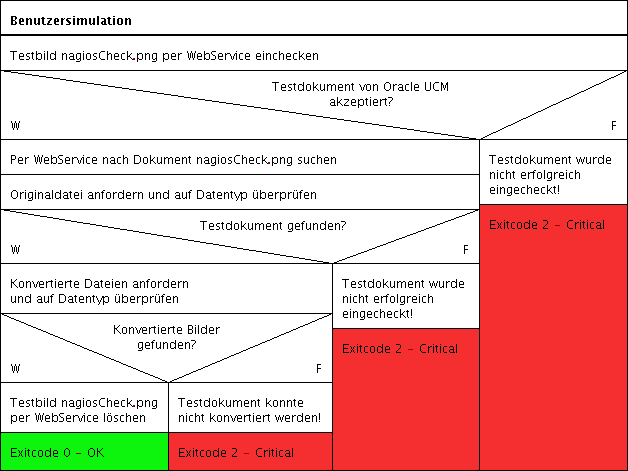
\includegraphics[width=0.85\textwidth]{bilder/Benutzersimulation.png}
		\caption{Geplanter Ablauf der Benutzersimulation}
		\label{user-sim}
\end{figure}

In diesem ersten Schritt wird durch das Einchecken eines Testbildes die Erreichbarkeit der Anwendung über das Netzwerk getestet.

Wenn die Übertragung des Bildes erfolgreich war, wird anschließend nach dem soeben eingecheckten Bild per Dateinamen gesucht um die Funktionalität der Indizierung zu kontrollieren.

Sollte das Bild gefunden werden, wird es vom Nagios-Server angefordert und auf seine Korrektheit überprüft.
Der gleiche Test wird mit den konvertieren Bildversionen durchgeführt, um die Funktion der Konvertierung zu überwachen.

Falls alle Tests erfolgreich waren, wird das Testbild und alle konvertierten Bilder vom \gls{OracleUCM}-Server gelöscht.
Bei den anderen Szenarien gibt das Plugin den Wert 2 für den Status \pictext{CRITICAL} zurück.
\newpage
Die Benutzersimulation wird durch zwei Plugins realisiert.

\paragraph{Einchecken eines Testbildes}
Das erste Plugin dient zum Einchecken des Testbildes.
Dabei ruft der Nagios-Server ein auf \gls{PHP}-basierendes Script auf.
In diesem Script wird die \gls{PHP}-Bibliothek nuSOAP eingebunden, damit man vereinfacht auf Web Services zugreifen kann.
Die Kommunikation zwischen Client und Server bei der Benutzung eines Web Services findet, wie im Kapitel \ref{webservice} beschrieben, im \gls{XML}-Format statt.
Um den Aufwand zu vermeiden diese \gls{XML}-Datei immer selbst zu erstellen, wird mit Hilfe der \gls{WSDL}-Datei auf dem \gls{OracleUCM}-Server die benötigten Parameter beim Aufruf eines Web Services von nuSOAP ausgelesen.

In der folgenden Abbildung werden aus der \gls{WSDL}-Datei alle möglichen Anforderungsparameter für den Web Service \textit{CheckInUniversal} gezeigt.

\begin{figure}[ht]
	\centering
	   \fbox{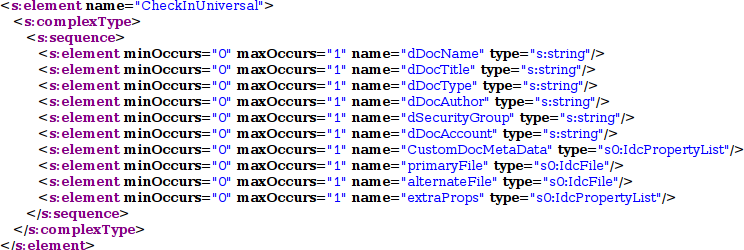
\includegraphics[width=0.85\textwidth]{bilder/wsdlscrn.png}}
		\caption{Anforderungsparameter für CheckInUniversal aus der WSDL-Datei}
		\label{wsdl1}
\end{figure}


%\begin{lstlisting}[captionpos=b, caption=Anforderungsparameter aus der WSDL-Datei, label=1stwsdl, breaklines = true, language=xml]
%<s:element name="CheckInUniversal">
% <s:complexType>
%  <s:sequence>
%   <s:element minOccurs="0" maxOccurs="1" name="dDocTitle" type="s:string"/>
%   <s:element minOccurs="0" maxOccurs="1" name="dDocType" type="s:string"/>
%   <s:element minOccurs="0" maxOccurs="1" name="dDocAuthor" type="s:string"/>
%   <s:element minOccurs="0" maxOccurs="1" name="dSecurityGroup" type="s:string"/>
%   <s:element minOccurs="0" maxOccurs="1" name="dDocAccount" type="s:string"/>
%   <s:element minOccurs="0" maxOccurs="1" name="primaryFile" type="s0:IdcFile"/>
%  </s:sequence>
% </s:complexType>
%</s:element>
%\end{lstlisting}

Im PHP-Script werden nach dem Einlesen dieser \gls{WSDL}-Datei und der Authentifizierung am \gls{OracleUCM}-Server die benötigten Parameter beim Aufruf des Web Services gesetzt und die Ausgabe des Servers ausgewertet.

\begin{lstlisting}[captionpos=b, caption=Anforderungsparameter des ersten Plugins, label=1stplugin, breaklines = true, language=PHP]
$soap = new soapclient($WSDL-URL,  //WSDL-Datei einlesen 
array('login' => $user, 'password' => $password)); //Authentifizierung am Oracle UCM-Server

//Aufruf des Web Services
$ergebnis = $soap->CheckInUniversal(array(
	'dDocAuthor'=>$user, //Autor des Bildes
	'dDocTitle'=>'testBild4nagios', //Titel des Bildes
	'dSecurityGroup'=>'private', //Sichtbarkeit des Bildes
	'dDocAccount'=>'NAGIOS/TEST', //Angabe einer Gruppe
	'dInDate'=>date("d.m.y H:i"), //Aktuelles Datum
	'dDocType'=>'Picture', //Dokumententyp
	'doFileCopy'=>'1', //Datei nur kopieren, nicht verschieben
	'dDocFormat'=>'image/png', //MIME-Type
	'primaryFile'=>array(
		'fileName'=>'testBild4nagios',
 		'fileContent'=>$content) //Byteweise eingelesenes Bild
));
[...]
//Auswertung der Antwort des Servers
if (ereg(' erfolgreich eingecheckt.', $output)) {
  echo('CHECKIN OK - '.$output);
  die(0); //Einchecken erfolgreich
} else {
 echo('CHECKIN CRITICAL - '.$output);
 die(2); //Einchecken fehlgeschlagen
}
\end{lstlisting}

Die Bilddatei muss für die Übertragung über \gls{HTTP} zuerst byteweise eingelesen werden und anschließend mit dem Base64-Algorithmus kodiert werden.
Dabei übernimmt die nuSOAP-Bibliothek die Base64-Enkodierung.

Der Ablauf dieses Plugins soll durch das folgende Schaubild verdeutlicht werden.
\begin{figure}[ht]
	\centering
	   \fbox{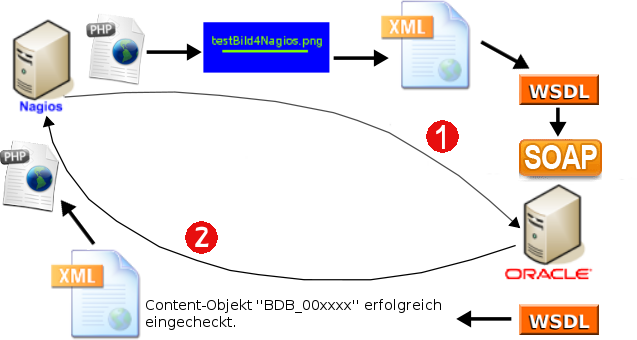
\includegraphics[width=0.85\textwidth]{bilder/wsdl.png}}
		\caption{Einchecken eines Testbildes}
		\label{usersim}
\end{figure}

\begin{enumerate}
\item Im ersten Schritt wird das \gls{PHP}-Script vom Nagios-Server aufgerufen und liest das Testbild ein. Anschließend verwendet es die \gls{WSDL}-Datei des Web Services um das entsprechende \gls{XML}-Dokument zu erstellen. Diese \gls{XML}-Datei wird anhand der nuSOAP-Bibliothek \gls{SOAP}-konform an den \gls{OracleUCM}-Servers gesendet.
\item Die \gls{XML}-basierende Rückantwort des Servers wird auch anhand der \gls{WSDL}-Datei erstellt und kann vom \gls{PHP}-Script ausgewertet werden.
\end{enumerate}


\paragraph{Validierung der Indizierung und Konvertierung}
Der zweite Teil der Benutzersimulation überprüft, ob das Testbild erfolgreich indiziert und konvertiert wurde.
Dabei verwendet es die gleichen Grundfunktionen wie das erste Plugin.
Jedoch wird anstatt dem Web Service \textit{CheckInUniversal} die \gls{WSDL}-Datei des Web Services \textit{AdvancedSearch} verwendet und aufgerufen.

\begin{lstlisting}[captionpos=b, caption=Überprüfen der Indizierung anhand einer Suchanfrage, label=2stplugin, breaklines = true, language=PHP]
$ergebnis = $soap->AdvancedSearch(
	'queryText'=>"dDocTitle <substring> `testBild4Nagios");
\end{lstlisting}

Durch diesen Aufruf wird anhand seines Titels nach einem zuvor eingechecktem Testbild gesucht.
Dadurch kann überprüft werden, ob das Bild korrekt vom Server angenommen und indiziert wurde.
In der Rückantwort des Servers befindet sich unter anderem die eindeutige Identifikationsnummer des Testbildes.
Diese Nummer wird für die Validierung der Konvertierung verwendet.
\begin{lstlisting}[captionpos=b, caption=Überprüfen der Indizierung anhand einer Suchanfrage, label=2stplugin, breaklines = true, language=PHP]
//Test des Originalbildes
$ergebnisGet = $soap->GetFileByID('dID'=>$dID);
[...]
if(!mb_eregi('PNG', $outputGetOrig))
{
        echo('SEARCH CRITICAL - Originalbild ist nicht im PNG Format!');
        die(2); //Originalbild korrupt
}
//Test der Thumbnailversion des Testbildes
$ergebnisGetThumbnail = $soap->GetFileByID(array('dID'=>$dID, 'rendition' => 'Thumbnail'));
[...]
if(!mb_eregi('JFIF', $outputGetThumbnail))
{
        echo('SEARCH CRITICAL - Thumbnailversion des Testbildes ist nicht im JPEG Format!');
        die(2); //Thumbnailversion korrupt
}
\end{lstlisting}

Sofern das Bild gefunden wurde, wird es vom Plugin anschließend angefordert und nach dem Dateityp untersucht.
%Die Konvertierung wird dadurch überprüft indem die konvertierten Versionen des Testbildes angefordert werden und wie das Originalbild auf einen gültigen Dateityp getestet werden.
%Die Konvertierung wird dadurch überprüft indem die konvertierten Versionen auf einen gültigen Dateityp getestet werden.
Für die Überprüfung auf den gültigen Datentyp wird direkt in den Bytecode der verschiedenen Versionen des Testbildes geschaut.

\begin{figure}[ht]
	\centering
	   \fbox{\subfigure[PNG-Bild]{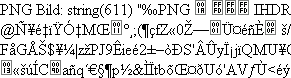
\includegraphics[scale=0.6]{bilder/eregi-png.png}} \quad \quad
	   \subfigure[JPEG-Bild]{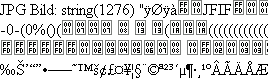
\includegraphics[scale=0.6]{bilder/jpg-eregi.png}}
	   }
		\caption{Bytecode von PNG- und JPEG-Bilddateien}
		\label{bytecode}
\end{figure}

Dabei wird für das Originalbild nach PNG und für die in JPEG konvertierten Versionen nach JFIF (JPEG File Interchange Format) geschaut.

Der Ablauf dieses Plugins ist dem ersten sehr ähnlich, wie Abbildung \ref{usersim2} zeigt.

\begin{figure}[ht]
	\centering
	   \fbox{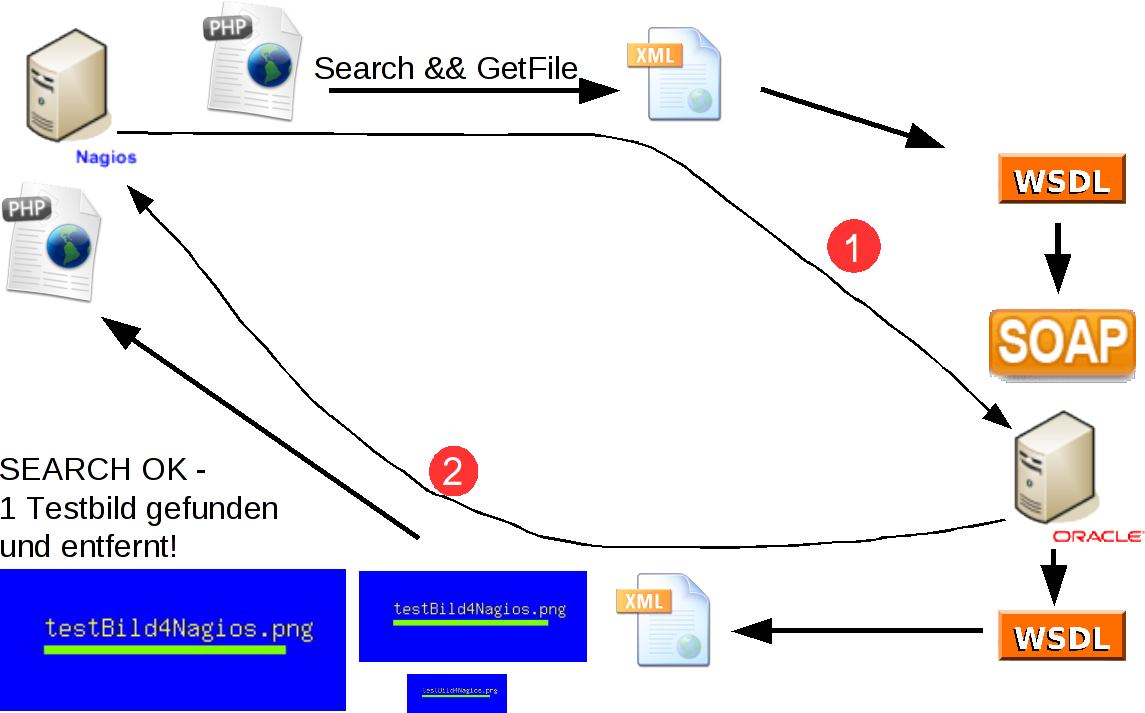
\includegraphics[width=0.85\textwidth]{bilder/wsdl-valid.png}}
		\caption{Validierung der Indizierung und Konvertierung}
		\label{usersim2}
\end{figure}

\begin{enumerate}
\item Zuerst wird die \gls{WSDL}-Datei für den Web Service \textit{AdvancedSearch} eingelesen. Eine Suchanfrage nach dem Testbild wird wieder über eine \gls{XML}-Datei an den Server gesendet. Wenn eine Datei gefunden wurde, wird das Originalbild und die konvertierten Versionen anhand der Identifikationsnummer angefordert.
\item Diese Bilder werden wieder byteweise innerhalb der \gls{XML}-Datei der Serverantwort an den Nagios-Server übertragen und auf ihre Korrektheit überprüft. Sollten alle bisherigen Tests ohne Probleme abgelaufen sein, wird das Testbild und die konvertierten Bilder vom Server entfernt.
\end{enumerate}

Damit nicht unnötiger Festplattenplatz durch die Testbilder verschwendet wird, sollen die Testbilder mit den konvertierten Version vom Server gelöscht werden.

Standardmäßig bietet \gls{OracleUCM} keinen Web Service zum Löschen von Dokumenten an.
Daher muss zunächst eine \gls{WSDL}-Datei dafür erstellt werden, siehe Abbildung \ref{cwsdl}.

\begin{figure}[ht]
	\centering
	   \fbox{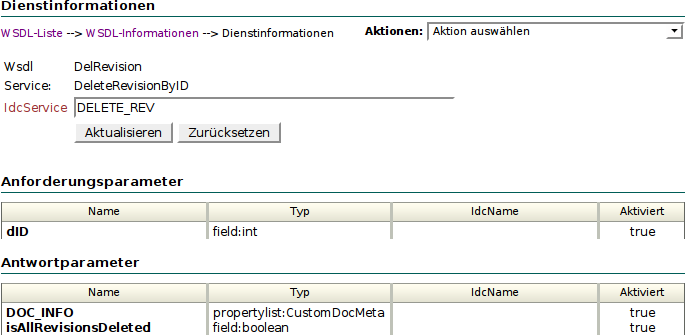
\includegraphics[width=0.85\textwidth]{bilder/cwsdl2.png}}
		\caption{Anlegen eines eigenen Web Services}
		\label{cwsdl}
\end{figure}


Der Name der \gls{WSDL}-Datei und des Web Services kann beliebig gewählt werden, solange als Service die entsprechende interne Bezeichnung zum Löschen von Dokumenten \pictext{DELETE\_REV} verwendet wird.\footnote{Quelle: \cite{Huff06} S. 379}
Um Zweideutigkeiten zu vermeiden, wird als Anforderungsparameter die eindeutige Identifikationsnummer verwendet.

Der eigene Web Service wird wie die anderen im Anschluss aufgerufen:

\begin{lstlisting}[captionpos=b, caption=Aufruf des eigenen Web Services, label=2stplugin2, breaklines = true, language=PHP]
$ergebnisDelete = $soap->DeleteRevisionByID('dID'=>$dID);
\end{lstlisting}
Die erstellten PHP-Dateien müssen noch Nagios als Befehl hinzugefügt werden.
\begin{lstlisting}[captionpos=b, caption=Befehldefinitionen der Benutzersimulation, label=phpdef, breaklines = true, language=sh]
#Einchecken eines Testbildes
define command{
        command_name    check_ucm_checkin
        command_line    /usr/lib/nagios/plugins/check_ucm/nagiosCheckin.php
        }
#Validierung der Indizierung und Konvertierung
define command{
        command_name    check_ucm_search
        command_line    /usr/lib/nagios/plugins/check_ucm/nagiosSearch.php
        }
\end{lstlisting}

Die Aufteilung der Benutzersimulation in zwei Nagios-Kommandos sorgt dafür, dass es keine Garantie für die Reihenfolge der Ausführung der Plugins gibt.
Aufgrund diese Asynchronität und dem Umstand, dass die Indizierung und Konvertierung des Testbildes abhängig von der Auslastung des \gls{OracleUCM}-Servers ist, wird die Anzahl der Ausführungen des Plugins für den Wechsel von Soft zum Hard State erhöht.

\begin{lstlisting}[captionpos=b, caption=Angepasste Servicedefinition für die Benutzersimulation, label=phpdef, breaklines = true, language=sh]
define service{
        use                     generic-service
        host_name               example.kit.edu
        service_description     Oracle UCM Search Delete
        max_check_attempts      8
        check_command           check_ucm_search
        }
\end{lstlisting}

%\begin{itemize}
%\item \url{http://www.w3schools.com/soap/default.asp} Web Services und SOAP
%\item \url{http://www.w3schools.com/wsdl/wsdl_summary.asp} WSDL
%\item max attempts bei Search erhöhen, da Auslastung der InboundRef -> möglichst keine/geringe False Positives -> auf Ausblick verweisen, Rahmenbedingungen müssen im Feld in der Praxis erst noch gefunden werden
%\end{itemize}